\documentclass{article}

\usepackage{mathtools}
\usepackage{bm}
\usepackage[margin=1.25in]{geometry}
\usepackage{courier}
\usepackage{color}
\usepackage{listings}
\usepackage{pdfpages}

\definecolor{dkgreen}{rgb}{0,0.6,0}
\definecolor{gray}{rgb}{0.5,0.5,0.5}

\newcommand{\blankpage}{
	\newpage
	\thispagestyle{empty}
	\mbox{}
	\newpage
}

\title{Optimization Methods, Project 2}
\date{2015/11/18}
\author{Matthew Grasinger}

\begin{document}
	
\lstset{language=Matlab,
	keywords={break,case,catch,continue,else,elseif,end,for,function,
		global,if,otherwise,persistent,return,switch,try,while},
	basicstyle=\ttfamily,
	keywordstyle=\color{blue},
	commentstyle=\color{gray},
	stringstyle=\color{dkgreen},
	numbers=left,
	numberstyle=\tiny\color{red},
	stepnumber=1,
	numbersep=10pt,
	backgroundcolor=\color{white},
	tabsize=4,
	showspaces=false,
	showstringspaces=false}
	
\pagenumbering{gobble}
\maketitle
\newpage
\tableofcontents
\newpage
\pagenumbering{arabic}

\section{Line Search: Golden Section}

\subsection{Objective}

The goal is to find the optimal step size given a current estimate of the parameters and a desired direction to explore.
Given $N$ points, the cost function that we are aiming to minimize is given by,

\begin{equation}
E = \sum_{i = 1}^{N} |y_i - a x_i - b|
\end{equation}

\noindent where $x_i$ and $y_i$ are the coordinates of the $i^{th}$ point and $a$ and $b$ are the parameters over which the cost function is being minimized.

The points can be found in Table \ref{table:points}.
The initial guess and direction of search are $\mathbf{a_0} = \begin{bmatrix} 1 & 1 \end{bmatrix}^T$ and $\mathbf{d} = \begin{bmatrix} 2 & 1 \end{bmatrix}^T$, respectively.

\begin{table}
\centering
\begin{tabular}{| c | c |}
	\hline
	$x_i$ & $y_i$ \\ \hline
	-2  & 1	  \\
	-1  & 3   \\
	0   & 5   \\
	1   & 7   \\
	2   & 9 \\
	\hline
\end{tabular}
\caption{Points in which to fit a straight line to}
\label{table:points}
\end{table}

\subsection{Source Code}

A function, \texttt{line\_search\_golden}, was created in MATLAB with the purpose of searching for the minimum of a unimodal, scalar function.
The function takes a function handle (for the function to be minimized), an initial range of search, a tolerance for which to search to, and a maximum number of iterations as input.
It returns the approximate minimum, the final range, the number of iterations performed, and whether or not the search converged, as output.

The cost function to be minimized was imlemented in terms of a MATLAB function, \linebreak \texttt{lin\_approx\_accum\_abs\_error}.

The source code for both functions are what follows.

\vspace{0.25in}
\begin{lstlisting}
%% line_search_golden.m

function [alpha, range, iters, converged] = ...
  line_search_golden(func_handle, init_range, eps, max_iters, plot_error)
%LINE_SEARCH_GOLDEN Perform line search using method of golden section
%
%   [alpha, range, iters, converged] = LINE_SEARCH_GOLDEN(func_handle, ...
%                                                         init_range,  ...
%                                                         eps,         ...
%                                                         max_iters,   ...
%                                                         plot_error)
%
%   Line search using method of golden section until the range is smaller 
%   than the tolerance provided by the input eps, or until the maximum 
%   number of iterations has been reached. Cost function is given by the 
%   handle func_handle.

rho = (sqrt(5) - 1) / 2;

if nargin < 5
  plot_error = false;
end

y = zeros(2, 1);
range = init_range;
converged = false;

a = range(2) - rho * (range(2) - range(1));
b = range(1) + rho * (range(2) - range(1));
y(1) = func_handle(a);
y(2) = func_handle(b);

if plot_error
  ranges = zeros(50, 2);
  ranges(1,:) = init_range;
  Es = zeros(50, 1);
  for iters = 1:max_iters
    if y(1) < y(2)
      Es(iters) = y(1);
      range(2) = b;
      b = a;
      a = range(2) - rho * (range(2) - range(1));
      y(2) = y(1);
      y(1) = func_handle(a);
    else
      Es(iters) = y(2);
      range(1) = a;
      a = b;
      b = range(1) + rho * (range(2) - range(1));
      y(1) = y(2);
      y(2) = func_handle(b);
    end

    if range(2) - range(1) < eps;
      converged = true;
      break;
    end
    
    ranges(iters+1,:) = range;
  end
  
  Es(iters+1) = min(y);
  xs = linspace(0, iters, iters+1);
  plot(xs, Es(1:iters+1));
  title('Error vs. Iterations');
  figure();
  
  hold on;
  for i=1:iters
    xs = linspace(ranges(i,1), ranges(i,2), 100);
    ys = ones(100, 1) * (i-1);
    plot(xs, ys);
  end
  title('Range at each Iteration');
else
  for iters = 1:max_iters-1
    if y(1) < y(2)
      range(2) = b;
      b = a;
      a = range(2) - rho * (range(2) - range(1));
      y(2) = y(1);
      y(1) = func_handle(a);
    else
      range(1) = a;
      a = b;
      b = range(1) + rho * (range(2) - range(1));
      y(1) = y(2);
      y(2) = func_handle(b);
    end

    if range(2) - range(1) < eps;
      converged = true;
      break;
    end
  end
end

if y(1) < y(2)
  alpha = a;
else
  alpha = b;
end

end


\end{lstlisting}

\vspace{0.25in}

\begin{lstlisting}
%% lin_approx_accum_abs_error.m

function error = lin_approx_accum_abs_error(X, a)
%LIN_APPROX_ACCUM_ABS_ERROR Accumulated absolute error for line of fit
%
%   error = LIN_APPROX_ACCUM_ABS_ERROR(X, a)
%   Sum of absolute values of differences between a linear approximation
%   given by a(1)*x + a(2) and actual data points in two dimensions

error = 0;
rows = size(X, 1);
for i=1:rows
  error = error + abs(X(i,2) - a(1)*X(i,1) - a(2));
end

end

\end{lstlisting}

\vspace{0.25in}

\subsection{Results}

The code executed and the resulting output of the \texttt{line\_search\_golden} function was,

\vspace{0.25in}

\begin{verbatim}
>> X = csvread('points.csv')

X =

-2     1
-1     3
0     5
1     7
2     9

>> x_0 = [1; 1];
>> d = [2; 1];
>> [alpha, range, iters, converged] = line_search_golden(...
     @(a) lin_approx_accum_abs_error(X, x_0 + a*d), ...
     [0; 2], 1e-4, 1000, true)

alpha =

1.2000


range =

1.2000
1.2001


iters =

21


converged =

1

\end{verbatim}

\vspace{0.25in}

\subsubsection{What is the new estimate of the parameters?}

The new estimate of the parameters is,

\begin{eqnarray*}
\mathbf{a} &= \begin{bmatrix} a \\ b \end{bmatrix} &= \mathbf{x_0} + \alpha \mathbf{d} \\
&&= \begin{bmatrix} 1 \\ 1 \end{bmatrix} + 1.2 \begin{bmatrix} 2 \\ 1 \end{bmatrix} \\
&&= \begin{bmatrix} 3.4 \\ 2.2 \end{bmatrix}
\end{eqnarray*}

\subsubsection{How many iterations did you expect to perform? How many did you end up needing?}

The golden ratio is given by $\phi = \frac{1 + \sqrt{5}}{2}$.
Line searching by golden section shrinks the range of search by $\phi-1$ after each iteration.
In order to narrow the range to less than or equal to $10^{-4}$ in length, the number of iterations expected to be performed are,

\begin{eqnarray*}
2 (\phi - 1)^N &=& 10^{-4} \\
\log(2) + N \log(\phi-1) &=& -4\\
N &=& \frac{-4 - \log(2)}{\log(\phi-1)}\\
N &=& 20.58
\end{eqnarray*}

\noindent where $N$ is the number of iterations.
Rounding up, $N$ becomes 21, which is exactly the number of iterations performed in the search.

\subsubsection{Plot the value of E at each iteration}

Plots of E at each iteration and the range of search at each iteration can be seen in Figures \ref{fig:error} and \ref{fig:range}, respectively.

\begin{figure}
	\centering
	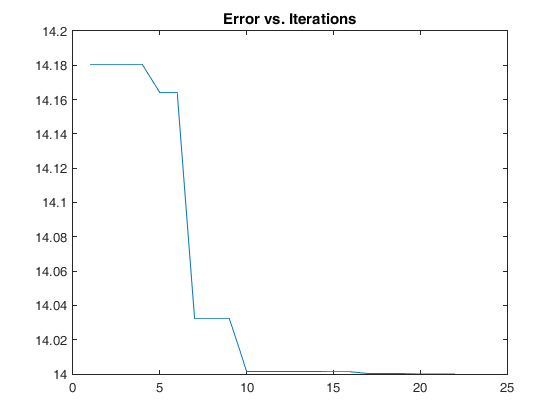
\includegraphics[width=0.75\linewidth]{error-vs-iterations}
	\caption{Minimum value of cost function after each iteration}
	\label{fig:error}
\end{figure}

\begin{figure}
	\centering
	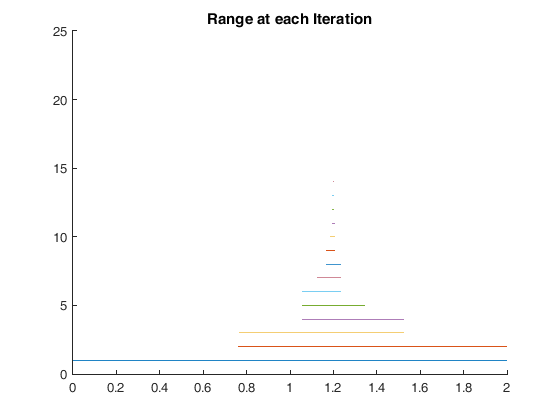
\includegraphics[width=0.75\linewidth]{range-at-each-iteration}
	\caption{Range at search for each iteration (y-value is the iteration number)}
	\label{fig:range}
\end{figure}

\end{document}
